% 原书PDF第40页4.2.3起至第54页4.3之前，含全部ASE应用图表。
\subsection{RNA-seq 数据的等位基因特异性表达差异分析}

识别等位基因特异性表达（ASE）的差异，对于整合基因组与转录组数据、揭示疾病机制十分重要。然而，可变的 ASE 具有复杂的表达模式。核苷酸序列变异会在基因、异构体、外显子、基因组位置和等位基因等不同层次，对表达变化产生不同影响。近年来，RNA-seq 这一高通量测序技术，为测量基因表达、刻画表达特征及揭示表达机制提供了有力工具，从而能够揭示复杂的表达模式。基于下一代测序的表达谱方法，可同时识别遗传多态性、定量 ASE、全面刻画转录组，并发现差异表达的等位基因。RNA-seq 正成为 ASE 研究的主要方法。

现有 RNA-seq 差异分析方法比较基因表达值的差异，试图准确估计基因、异构体和等位基因特异性表达值（Trapnell et al. 2013）。估计的准确性在很大程度上依赖于所假定的模型。由于等位基因特异性的可变剪接、转录起始与终止位点、多聚腺苷酸化，以及自然选择或其他未知机制（Skelly et al. 2011），不同核苷酸与 SNP 之间存在显著的表达变异。基因、外显子、异构体、核苷酸和 SNP 等多层次的表达模式极为复杂，难以甚至不可能完整建模。

本节主要介绍用于检验两种条件间 ASE 显著差异的双变量函数主成分分析（bivariate functional principal component analysis，BFPCA）。它允许 ASE 水平随 SNP 变化，能够考虑复杂的 ASE 模式。现有 ASE 识别方法往往要求已知单倍型，但 NGS 数据中的单倍型数量极大，含罕见变异的单倍型估计误差很高。为避免单倍型推断，我们引入 ASE 函数向量：将基因内每个 SNP 的三种基因型对应的读段数定义为基因组位置的函数。ASE 函数为随机函数。将单变量 FPCA 扩展为多变量 FPCA，利用 Karhunen–Loève 分解把随机函数展开为正交函数主成分，进而构造基于 BFCA 的新统计量，检验两种条件间的 ASE 显著差异。该方法比较不同实验条件下 ASE 函数的主成分得分差异，而非 ASE 总体水平的差异，或用于拟合 RNA-seq 实测 ASE 的模型参数差异。因此，基于 BFPCA 的统计方法允许 ASE 水平随 SNP 改变。

\subsubsection{用于检验 ASE 或差异表达的单变量 FPCA}
简要介绍基于 FPCA 的 ASE 或差异表达检验统计量。表达函数已在第4.2.2节定义。将条件1的 $X_i(t)$ 与条件2的 $Y_i(t)$ 合并，用于估计正交归一的主成分函数 $\phi_j(t)$（15）。由 Karhunen–Loève 展开，
\[
X_i(t)=\sum_{j=1}^{k}\xi_{ij}\beta_j(t),\qquad
Y_i(t)=\sum_{j=1}^{k}\eta_{ij}\beta_j(t),
\]
其中
\[
\xi_{ij}=\int_T X_i(t)\beta_j(t)\,dt,\qquad
\eta_{ij}=\int_T Y_i(t)\beta_j(t)\,dt.
\]
$\xi_{ij}$ 与 $\eta_{ij}$ 是均值为零、方差为 $\lambda_j$ 的不相关随机变量，且 $\sum_j\lambda_j<\infty$。以 $\bar\xi_j$ 与 $\bar\eta_j$ 分别表示条件1、条件2中主成分得分的均值。检验两种条件间基因差异表达或 ASE 的统计量定义为
\[
T_{\mathrm{FPC}}=\frac1{\dfrac1{n_A}+\dfrac1{n_G}}
\sum_{j=1}^{k}\frac{(\bar\xi_j-\bar\eta_j)^2}{S_j},
\]
其中
\[
S_j=\frac1{n_A+n_G-2}\left[\sum_{i=1}^{n_A}(\xi_{ij}-\bar\xi_j)^2
+\sum_{i=1}^{n_G}(\eta_{ij}-\bar\eta_j)^2\right].
\]
在两种条件间基因无差异表达或 ASE 的原假设下，$T_{\mathrm{FPC}}$ 渐近服从中心 $\chi^2_{(k)}$ 分布。

\subsubsection{用双变量函数主成分分析研究等位基因特异性差异表达}
\bookdeepheading{paragraph}{4.2.3.2.1}{等位基因表达函数向量的定义}
设 $t$ 为基因内某 SNP 的基因组位置，$T$ 为待检验基因的长度。考虑病例与对照两种条件，假设位于 $t$ 的 SNP 有两个等位基因。对于病例组第 $i$ 名个体，定义 $x_{i1}(t)$、$x_{i2}(t)$ 分别为该 SNP 的等位基因 $A$、$a$ 所产生的读段数，并令 $\mathbf x_i(t)=[x_{i1}(t),x_{i2}(t)]^T$。类似地，可定义对照组第 $j$ 名个体的 $\mathbf y_j(t)$。

\bookdeepheading{paragraph}{4.2.3.2.2}{将 RNA-seq 的 ASE 分析表述为双变量函数主成分分析}
设 $\boldsymbol\beta(t)=[\beta_1(t),\beta_2(t)]^T$ 为基函数向量，将内积定义为各分量内积之和：
\[
\begin{aligned}
f_i&=\langle\mathbf x_i,\boldsymbol\beta\rangle
=\langle x_{i1},\beta_1\rangle+\langle x_{i2},\beta_2\rangle\\
&=\int_T x_{i1}(t)\beta_1(t)\,dt+\int_T x_{i2}(t)\beta_2(t)\,dt
=\int_T=\boldsymbol\beta^T(t)\mathbf x_i(t)\,dt.
\end{aligned}
\]
由随机积分的方差公式，
\[
\Var(f_i)=\int_T\int_T\boldsymbol\beta^T(s)R(s,t)\boldsymbol\beta(t)\,ds\,dt,
\]
其中 $R(s,t)$ 为矩阵值协方差函数，可写为 $[R(s,t)]_{ij}=R_{ij}(s,t)$，即第 $ij$ 个元素为 $x_i(t)$ 与 $x_j(t)$ 的协方差函数。令
\[
\lVert\boldsymbol\beta\rVert_2=\int_T\boldsymbol\beta^T(t)\boldsymbol\beta(t)\,dt.
\]
函数主成分要在约束 $\lVert\boldsymbol\beta\rVert_2=1$ 下，最大化 $f_i$ 的方差：
\begin{equation}
\begin{aligned}
\max_{\boldsymbol\beta}\quad&\int_T\int_T
\boldsymbol\beta^T(s)R(s,t)\boldsymbol\beta(t)\,ds\,dt\\
\text{s.t.}\quad&\int_T\boldsymbol\beta^T(t)\boldsymbol\beta(t)\,dt=1.
\end{aligned}
\tag{4.112}
\end{equation}
利用 Lagrange 乘子，将约束优化问题 (4.112) 转化为无约束问题：
\[
\begin{aligned}
\max_{\boldsymbol\beta}\quad F(\boldsymbol\beta,\lambda)
={}&\int_T\int_T\boldsymbol\beta^T(s)R(s,t)\boldsymbol\beta(t)\,ds\,dt\\
&+\lambda\left(1-\int_T\boldsymbol\beta^T(t)\boldsymbol\beta(t)\,dt\right).
\end{aligned}
\]
令 $F(\boldsymbol\beta,\lambda)$ 的微分为零，得到
\begin{equation}
2\int_T\int_T\boldsymbol\beta^T(s)R(s,t)\,\partial\boldsymbol\beta(t)\,ds\,dt
-2\lambda\int_T\boldsymbol\beta^T(t)\boldsymbol\beta(t)\,dt=0.
\tag{4.113}
\end{equation}
由于式 (4.113) 必须对任意 $\partial\boldsymbol\beta(t)$ 成立，因而对所有 $t$，必须满足积分特征方程
\begin{equation}
\int_T R(t,s)\boldsymbol\beta(s)\,ds=\lambda\boldsymbol\beta(t).
\tag{4.114}
\end{equation}
这就是最优性条件。

假设在某区间内观测了 $n$ 个样本，将基因组位置 $t$ 处的全部观测写为矩阵
\[
X(t)=[\mathbf x_1(t),\mathbf x_2(t)]
=\begin{bmatrix}x_{11}(t)&x_{12}(t)\\\vdots&\vdots\\x_{n1}(t)&x_{n2}(t)\end{bmatrix}.
\]
将各样本的标量分量函数按基函数展开，得到
\[
\begin{aligned}
X(t)&=[Z_1\boldsymbol\Phi(t),Z_2\boldsymbol\Phi(t)]\\
&=[Z_1,Z_2]\begin{bmatrix}\boldsymbol\Phi(t)&0\\0&\boldsymbol\Phi(t)\end{bmatrix}
=Z(I_2\otimes\boldsymbol\Phi(t)),
\end{aligned}
\]
其中系数矩阵和基函数向量分别为
\[
Z_j\quad\begin{bmatrix}Z_{1j}^1&\cdots&Z_{1j}^k\\\vdots&\ddots&\vdots\\Z_{nj}^1&\cdots&Z_{nj}^k\end{bmatrix},
\qquad
\boldsymbol\Phi(t)=\begin{bmatrix}\phi_1(t)\\\vdots\\\phi_k(t)\end{bmatrix}.
\]
$I_2$ 为二维单位矩阵，$\otimes$ 表示矩阵的 Kronecker 积。于是，方差估计为
\[
\begin{aligned}
R(s,t)&\approx\frac1n X(s)^TX(t)\\
&=\frac1n(I_2\otimes\boldsymbol\Phi(s))^TZ^TZ(I_2\otimes\boldsymbol\Phi(t)).
\end{aligned}
\]
假设用相同的基函数 $\boldsymbol\Phi(t)$ 近似特征函数 $\boldsymbol\beta(t)$：
\[
\begin{aligned}
\boldsymbol\beta(t)&=[\beta_1(t),\beta_2(t)]^T
=[B_1^T\boldsymbol\Phi(t),B_2^T\boldsymbol\Phi(t)]^T\\
&=(I_2\otimes\boldsymbol\Phi^T(t))B,\qquad B=[B_1^T,B_2^T]^T.
\end{aligned}
\]
将其代入最优性条件 (4.114)，得到
\begin{equation}
\frac1n(I_2\otimes\boldsymbol\Phi^T(t))Z^TZB
=\lambda(I_2\otimes\boldsymbol\Phi^T(t))B.
\tag{4.115}
\end{equation}
若 $\boldsymbol\Phi(t)$ 正交归一，由于式 (4.115) 对任意 $t$ 成立，式 (4.114) 意味着
\[
\frac1n Z^TZB=\lambda B,
\]
即
\begin{equation}
\frac1n\begin{bmatrix}Z_1^TZ_1&Z_1^TZ_2\\Z_2^TZ_1&Z_2^TZ_2\end{bmatrix}
\begin{bmatrix}B_1\\B_2\end{bmatrix}
=\lambda\begin{bmatrix}B_1\\B_2\end{bmatrix}.
\tag{4.116}
\end{equation}
设 $B^j\;\begin{bmatrix}B_1^j\\B_2^j\end{bmatrix}$ 为式 (4.116) 的第 $j$ 个特征向量，则特征函数为
\begin{equation}
\boldsymbol\beta_j(t)\quad
\begin{bmatrix}\boldsymbol\Phi^T(t)B_1^j\\\boldsymbol\Phi^T(t)B_2^j\end{bmatrix}
=\begin{bmatrix}\beta_{j1}(t)\\\beta_{j2}(t)\end{bmatrix}.
\tag{4.117}
\end{equation}
因此，在基函数正交归一时，可由 $Z^TZ/n$ 计算特征函数的系数。

将 $\mathbf x_i(t)$ 按特征函数展开：
\[
\mathbf x_i(t)=\sum_{j=1}^{J}\xi_{ij}\boldsymbol\beta_j(t).
\]
第 $i$ 名个体等位基因表达函数的主成分得分可计算为
\begin{equation}
\xi_{ij}=\langle\mathbf x_i(t),\boldsymbol\beta_j(t)\rangle
=\sum_{k=1}^{2}\int x_{ik}(t)\beta_{jk}(t)\,dt
=\xi_{ij}^{(1)}+\xi_{ij}^{(2)},
\tag{4.118}
\end{equation}
其中
\[
\xi_{ij}^{(1)}=\int_T x_{i1}(t)\beta_{j1}(t)\,dt,\qquad
\xi_{ij}^{(2)}=\int_T x_{i2}(t)\beta_{j2}(t)\,dt.
\]

综上，计算函数主成分得分的算法如下。对每名个体定义二维等位基因表达曲线，分别考虑主要与次要等位基因。主要等位基因的展开为 $X_1(t)=Z_1\boldsymbol\Phi(t)$，次要等位基因为 $X_2(t)=Z_2\boldsymbol\Phi(t)$。定义矩阵 $Z=[Z_1\;Z_2]$，求解特征方程 (4.116)，得到特征向量，并构造特征函数
\[
\boldsymbol\beta_j(t)=\begin{bmatrix}\boldsymbol\Phi^T(t)B_1^j\\\boldsymbol\Phi^T(t)B_2^j\end{bmatrix}
=\begin{bmatrix}\beta_{j1}(t)\\\beta_{j2}(t)\end{bmatrix}.
\]
利用式 (4.118)，得到
\[
\xi_{ij}=\xi_{ij}^{(\mathrm{major})}+\xi_{ij}^{(\mathrm{minor})}.
\]

\bookdeepheading{paragraph}{4.2.3.2.3}{检验统计量}
与前一节类似，通过比较函数主成分得分构造差异 ASE 检验统计量。用式 (4.118) 分别计算条件1与条件2中的主成分得分
\[
\xi_{ij}=\xi_{ij}^{(\mathrm{major})}+\xi_{ij}^{(\mathrm{minor})},\qquad
\eta_{ij}=\eta_{ij}^{(\mathrm{major})}+\eta_{ij}^{(\mathrm{minor})},
\]
并以 $\bar\xi_j$、$\bar\eta_j$ 表示其均值。两种条件间差异 ASE 的检验统计量定义为
\[
T_{\mathrm{BFPC}}=\frac1{\dfrac1{n_A}+\dfrac1{n_G}}
\sum_{j=1}^{k}\frac{(\bar\xi_j-\bar\eta_j)^2}{S_j},
\]
其中
\[
S_j=\frac1{n_A+n_G-2}\left[\sum_{i=1}^{n_A}(\xi_{ij}-\bar\xi_j)^2
+\sum_{i=1}^{n_G}(\eta_{ij}-\bar\eta_j)^2\right],
\]
$k$ 为函数主成分个数。在两种条件间 ASE 无差异的原假设下，$T_{\mathrm{BFPC}}$ 渐近服从中心 $\chi^2_{(k)}$ 分布。

\Needspace{9\baselineskip}
\subsubsection{真实数据应用}
\bookdeepheading{paragraph}{4.2.3.3.1}{数据集}
为说明应用，将所提出的 BFPCA 用于一项精神分裂症 RNA-seq 研究，以及 TCGA 的卵巢癌 RNA-seq 数据。前者对31个精神分裂症样本与26个正常样本的 mRNA 测序；后者包括233个高级别严重型卵巢腺癌肿瘤样本，其中163个对治疗敏感、70个耐药。精神分裂症研究中的 RNA 样本取自死后脑组织，脑区为前扣带皮层，也称 Brodmann 24区。数据由 IlluminaHiSeq 平台产生，以 SeqWare Pipeline 项目进行预处理。剔除 SNP 数少于10的基因后，共分析11266个基因。

TCGA 卵巢癌项目同样使用 IlluminaHiSeq 平台。获得233名卵巢癌患者的原始 Bam 数据集，生成表达曲线谱，其中163名患者对化疗敏感、70名耐药。TCGA 委员会（2011）规定：若患者在六个月内复发，则判为铂类耐药；若无铂间期不少于六个月，且无进展或复发证据，并且自末次初始铂类治疗起随访至少六个月，则判为敏感。剔除 SNP 数少于10的基因后，共分析15104个基因。

\bookdeepheading{paragraph}{4.2.3.3.2}{差异 ASE 分析}
一个基因内全部 SNP 的两个等位基因读段计数形成两条表达谱。当 SNP 在基因内密集分布时，称其为 ASE 曲线或函数。对每个基因定义二维 ASE 函数向量，以这两条曲线为分量函数。分别对精神分裂症与正常样本，或卵巢癌治疗敏感与耐药肿瘤样本定义 ASE 函数向量。当两种条件间 ASE 存在显著差异时，可观察到 ASE 曲线的显著差异。因此，ASE 差异检验可以表述为两种条件间 ASE 曲线的差异检验。曲线维数很高，故用 FPCA 降维，再比较两组曲线的主成分得分，检验 ASE 显著差异。

精神分裂症与卵巢癌研究中检验的基因总数分别为11226与1871。Bonferroni 校正后的全基因组显著性阈值分别为 $4.44\times10^{-6}$ 与 $2.67\times10^{-5}$。共识别出16个在精神分裂症与正常样本间具有显著 ASE 差异的基因（表4.7）。卵巢癌研究中，没有差异 ASE 基因达到全基因组显著性；表4.8列出了治疗敏感与耐药样本间差异 ASE 检验的前10个基因及其 $P$ 值。
\begin{table}[htbp]
\centering\small
\origtable{7}{前16个差异 ASE 基因：精神分裂症与正常样本间差异表达，以及组内 ASE 检验的 $P$ 值}
\begin{tabular}{lrrr}
\toprule
&\multicolumn{3}{c}{$P$ 值}\\
\cmidrule(lr){2-4}
基因&差异 ASE&正常&精神分裂症\\
\midrule
SLC13A3&1.43E-08&1.71E-02&1.16E-07\\
TTF1&4.43E-08&2.86E-06&2.99E-13\\
AC019205&1.15E-07&4.82E-07&\textnormal{<1.0E-17}\\
PSMA5&2.14E-07&1.22E-03&1.17E-09\\
ANXA4&3.02E-07&2.84E-03&9.66E-06\\
LRRTM3&4.12E-07&3.46E-04&5.39E-10\\
FAM123A&5.82E-07&4.56E-06&\textnormal{<1.0E-17}\\
MAGI1&6.96E-07&1.70E-08&\textnormal{<1.0E-17}\\
XRN2&8.70E-07&6.22E-06&1.87E-14\\
KIF2A&1.49E-06&3.25E-08&4.22E-15\\
NUDT15&1.85E-06&4.71E-03&1.09E-11\\
ZNF815&1.87E-06&8.52E-05&6.81E-11\\
KALRN&2.09E-06&2.34E-07&1.47E-12\\
RRP15&2.46E-06&2.98E-07&1.89E-15\\
ST3GAL5&3.21E-06&5.25E-06&3.20E-13\\
CTNNAL1&3.67E-06&3.50E-06&8.97E-13\\
\bottomrule
\end{tabular}
\end{table}

\begin{table}[htbp]
\centering\small
\origtable{8}{卵巢癌前10个差异 ASE 基因：治疗敏感与耐药样本间差异 ASE，以及组内 ASE 检验的 $P$ 值}
\begin{tabular}{lrrr}
\toprule
&\multicolumn{3}{c}{$P$ 值}\\
\cmidrule(lr){2-4}
基因&差异 ASE&耐药&敏感\\
\midrule
PARP14&1.55E-04&\textnormal{<1.00E-17}&1.51E-04\\
DMTF1&4.13E-04&\textnormal{<1.00E-17}&2.44E-08\\
DDX60L, SNORA51&7.17E-04&\textnormal{<1.00E-17}&4.81E-08\\
SULT6B1, CEBPZ&8.07E-04&\textnormal{<1.00E-17}&3.38E-07\\
CEP89&1.13E-03&\textnormal{<1.00E-17}&1.58E-06\\
PDE4DIP&2.09E-03&\textnormal{<1.00E-17}&1.14E-05\\
RNPEP,ELF3&2.44E-03&\textnormal{<1.00E-17}&1.78E-15\\
RP4-758J18.9&2.67E-03&3.23E-02&2.59E-01\\
RQCD1&2.68E-03&4.33E-15&1.74E-03\\
COL18A1, SLC19A1&2.82E-03&3.00E-13&1.38E-05\\
\bottomrule
\end{tabular}
\end{table}


\bookdeepheading{paragraph}{4.2.3.3.3}{差异 ASE 的特征}
差异 ASE 包括两个部分：第一，存在 ASE，即表达依赖于等位基因；第二，ASE 在两种条件间有差异。差异 ASE 中，可以观察到每组内部（精神分裂症或正常、治疗敏感或耐药）两个等位基因在各 SNP 上的读段计数差异，以及对同一等位基因而言，两种条件间各 SNP 读段计数的差异。NGS 数据可产生许多单倍型，当个体数量很大时，测量群体中个体父源与母源单倍型的表达很困难，甚至不可能。这里通过统计每个基因内各 SNP 的每个等位基因读段数，对 ASE 进行定量。

图4.14与图4.15分别展示了 SLC13A3 主要与次要等位基因的表达曲线，该基因在精神分裂症与正常样本间有显著 ASE 差异。图4.16与图4.17分别展示了卵巢癌研究中 PARP14 主要与次要等位基因的 RNA-seq 表达曲线，该基因在治疗耐药与敏感样本间有 ASE 差异。
\begin{figure}[htbp]
\centering
\begin{tikzpicture}[x=1cm,y=1cm]
\node[anchor=south west,inner sep=0] at (0,0) {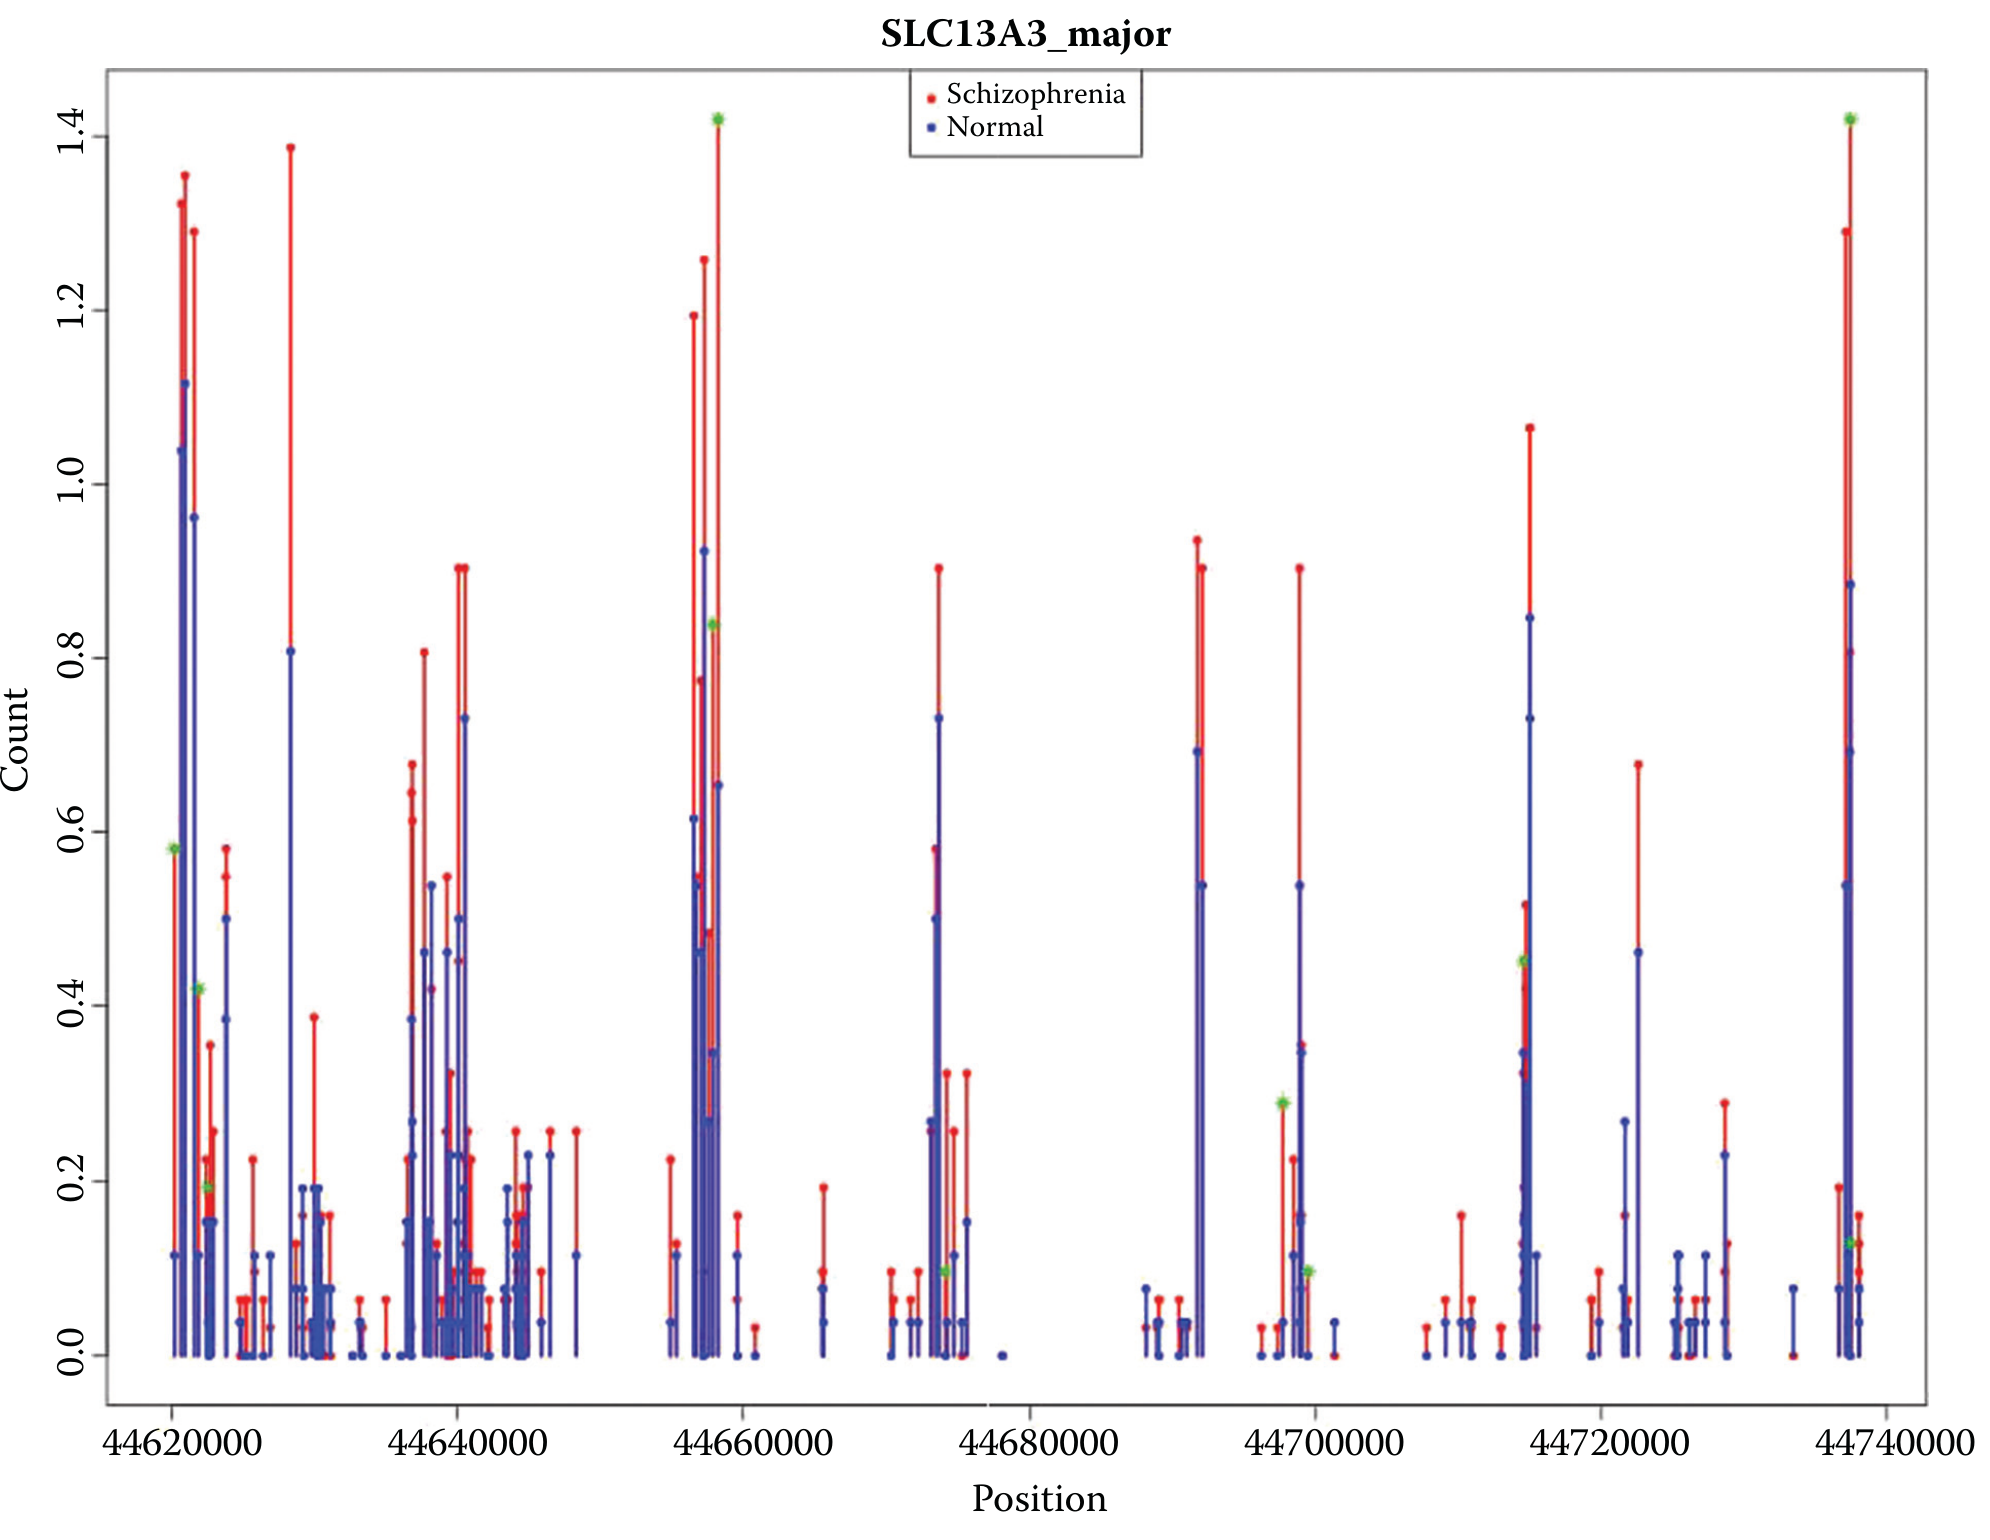
\includegraphics[width=12.0cm]{figures/ch04a_fig14_data.png}};
\fill[white] (5.6838,8.5975) rectangle (6.8152,8.8284);
\node[inner sep=0pt,fill=white,rotate=0,font=\fontsize{6}{8}\selectfont] at (6.2495,8.7130) {精神分裂症};
\fill[white] (5.6838,8.3947) rectangle (6.3195,8.6256);
\node[inner sep=0pt,fill=white,rotate=0,font=\fontsize{6}{8}\selectfont] at (6.0016,8.5101) {正常};
\fill[white] (-0.1054,4.4797) rectangle (0.3708,5.1653);
\node[inner sep=0pt,fill=white,rotate=90,font=\fontsize{8}{8}\selectfont] at (0.0652,4.8225) {计数};
\fill[white] (5.8321,0.0904) rectangle (6.7057,0.3816);
\node[inner sep=0pt,fill=white,rotate=0,font=\fontsize{8}{8}\selectfont] at (6.2689,0.2360) {位置};
\fill[white] (5.2844,8.9268) rectangle (7.0899,9.2180);
\node[inner sep=0pt,fill=white,rotate=0,font=\fontsize{8}{8}\selectfont] at (6.1872,9.0724) {SLC13A3：主要等位基因};
\end{tikzpicture}
\origfig{14}{基因 SLC13A3 主要等位基因的差异表达。}
\label{fig:ch04a-14}
\end{figure}

\begin{figure}[htbp]
\centering
\begin{tikzpicture}[x=1cm,y=1cm]
\node[anchor=south west,inner sep=0] at (0,0) {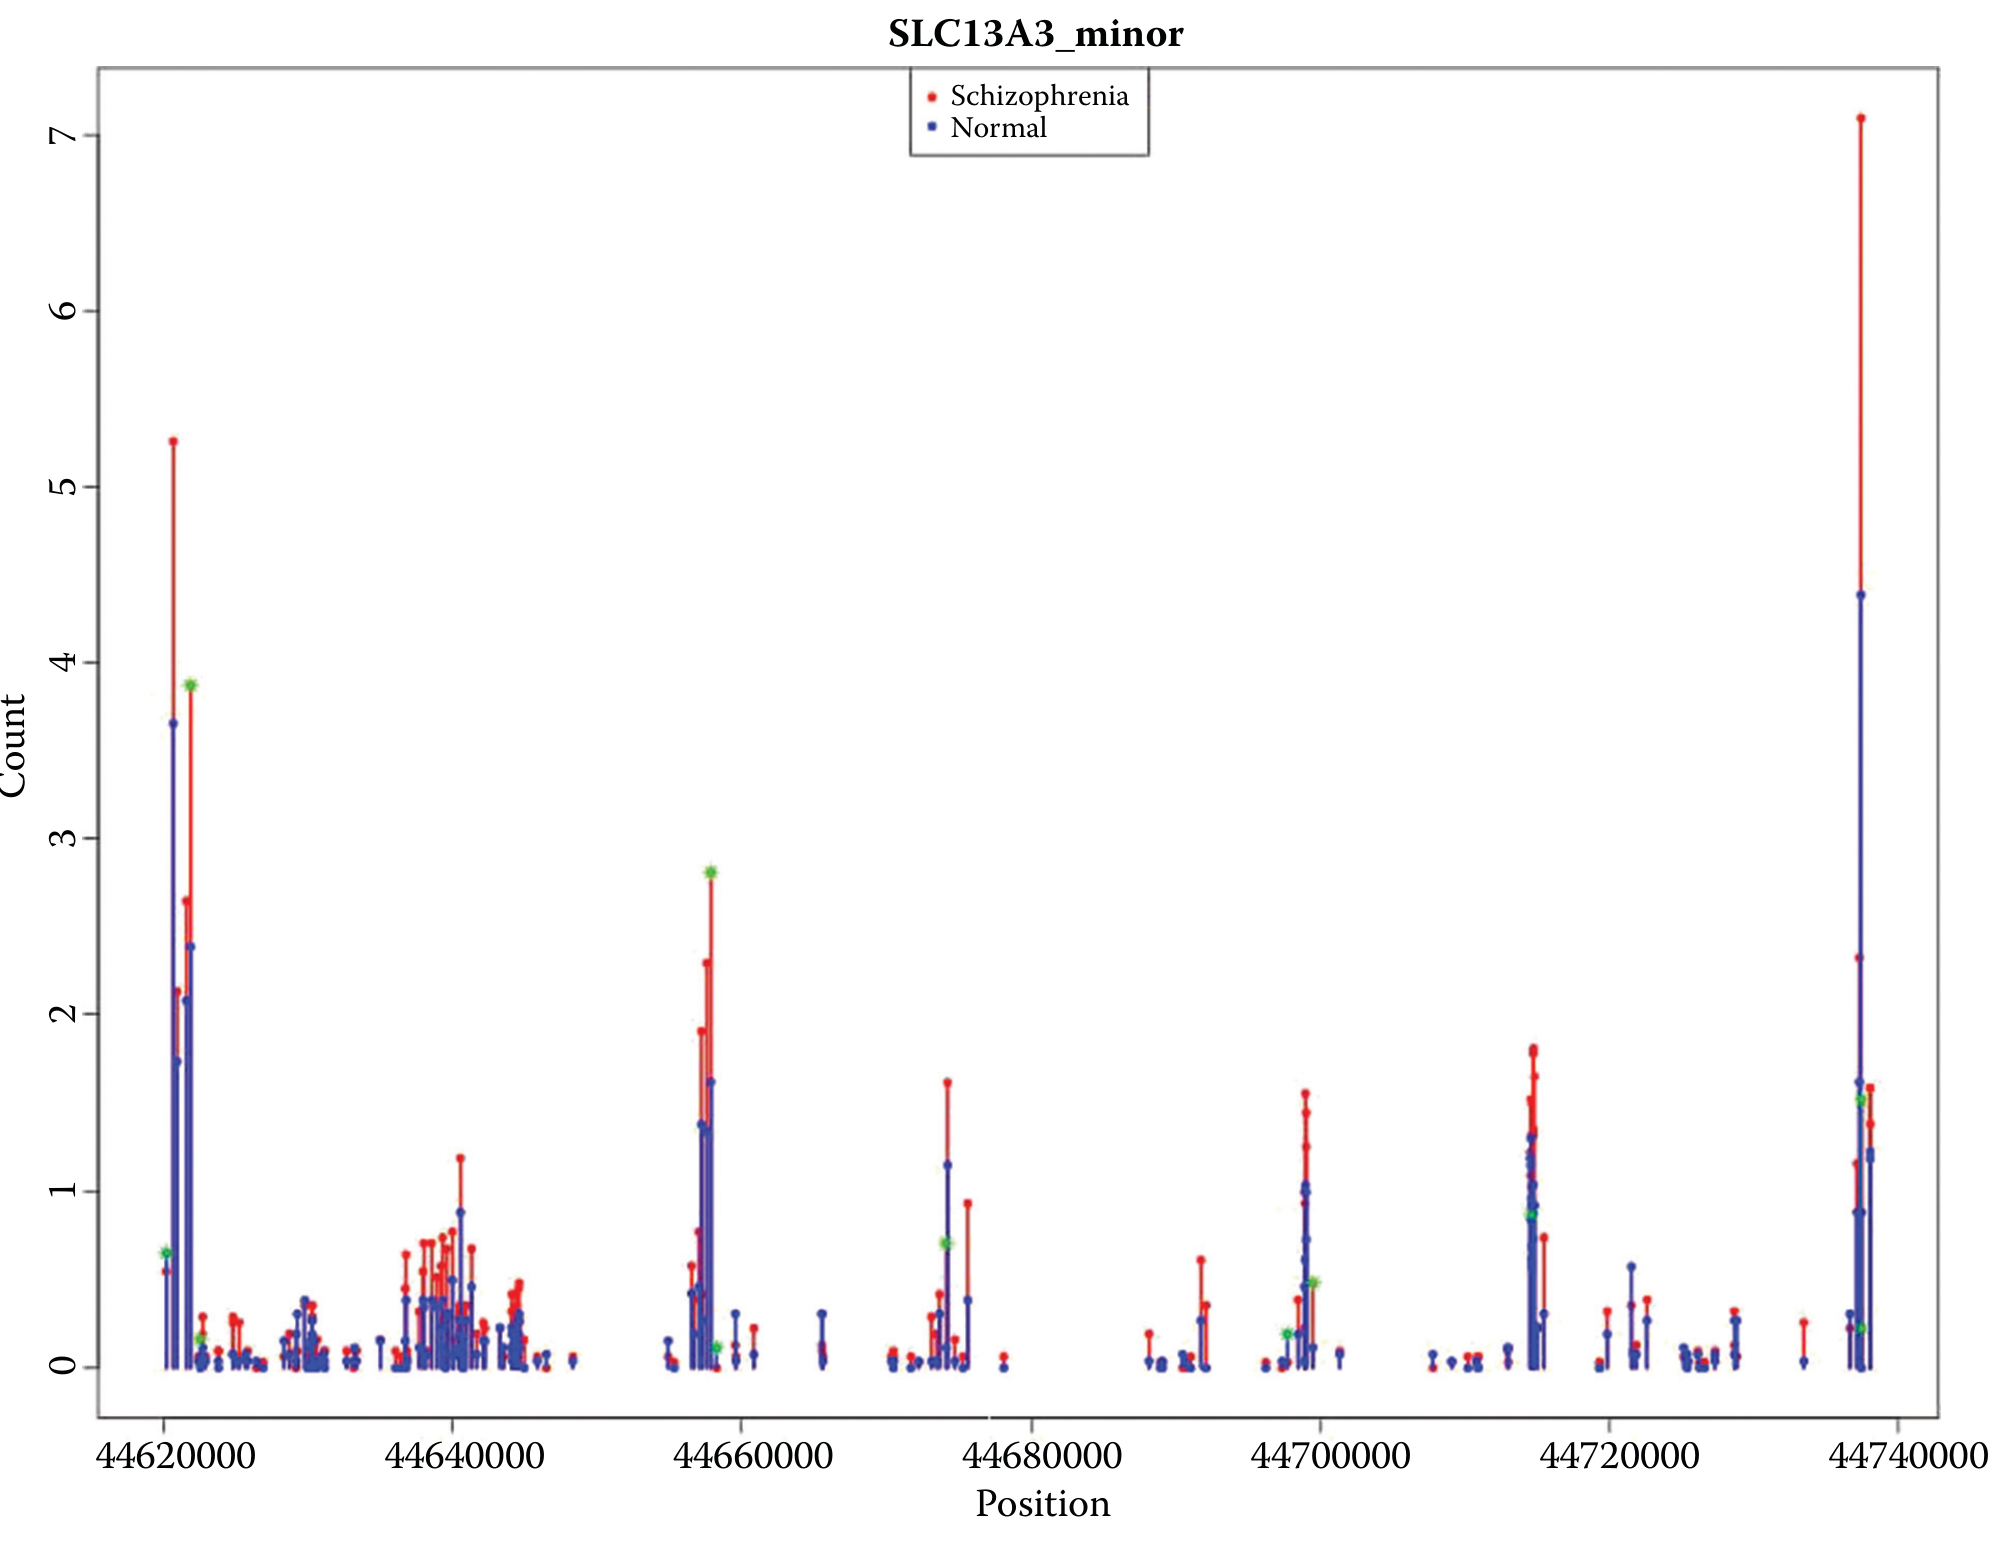
\includegraphics[width=12.0cm]{figures/ch04a_fig15_data.png}};
\fill[white] (5.6775,8.5683) rectangle (6.8042,8.7983);
\node[inner sep=0pt,fill=white,rotate=0,font=\fontsize{6}{8}\selectfont] at (6.2409,8.6833) {精神分裂症};
\fill[white] (5.3035,8.9120) rectangle (7.1288,9.2020);
\node[inner sep=0pt,fill=white,rotate=0,font=\fontsize{8}{8}\selectfont] at (6.2162,9.0570) {SLC13A3：次要等位基因};
\fill[white] (5.6775,8.3801) rectangle (6.3104,8.6101);
\node[inner sep=0pt,fill=white,rotate=0,font=\fontsize{6}{8}\selectfont] at (5.9939,8.4951) {正常};
\fill[white] (-0.1235,4.4508) rectangle (0.3515,5.1332);
\node[inner sep=0pt,fill=white,rotate=90,font=\fontsize{8}{8}\selectfont] at (0.0465,4.7920) {计数};
\fill[white] (5.8239,0.0903) rectangle (6.6934,0.3803);
\node[inner sep=0pt,fill=white,rotate=0,font=\fontsize{8}{8}\selectfont] at (6.2586,0.2353) {位置};
\end{tikzpicture}
\origfig{15}{基因 SLC13A3 次要等位基因的差异表达。}
\label{fig:ch04a-15}
\end{figure}

\begin{figure}[htbp]
\centering
\begin{tikzpicture}[x=1cm,y=1cm]
\node[anchor=south west,inner sep=0] at (0,0) {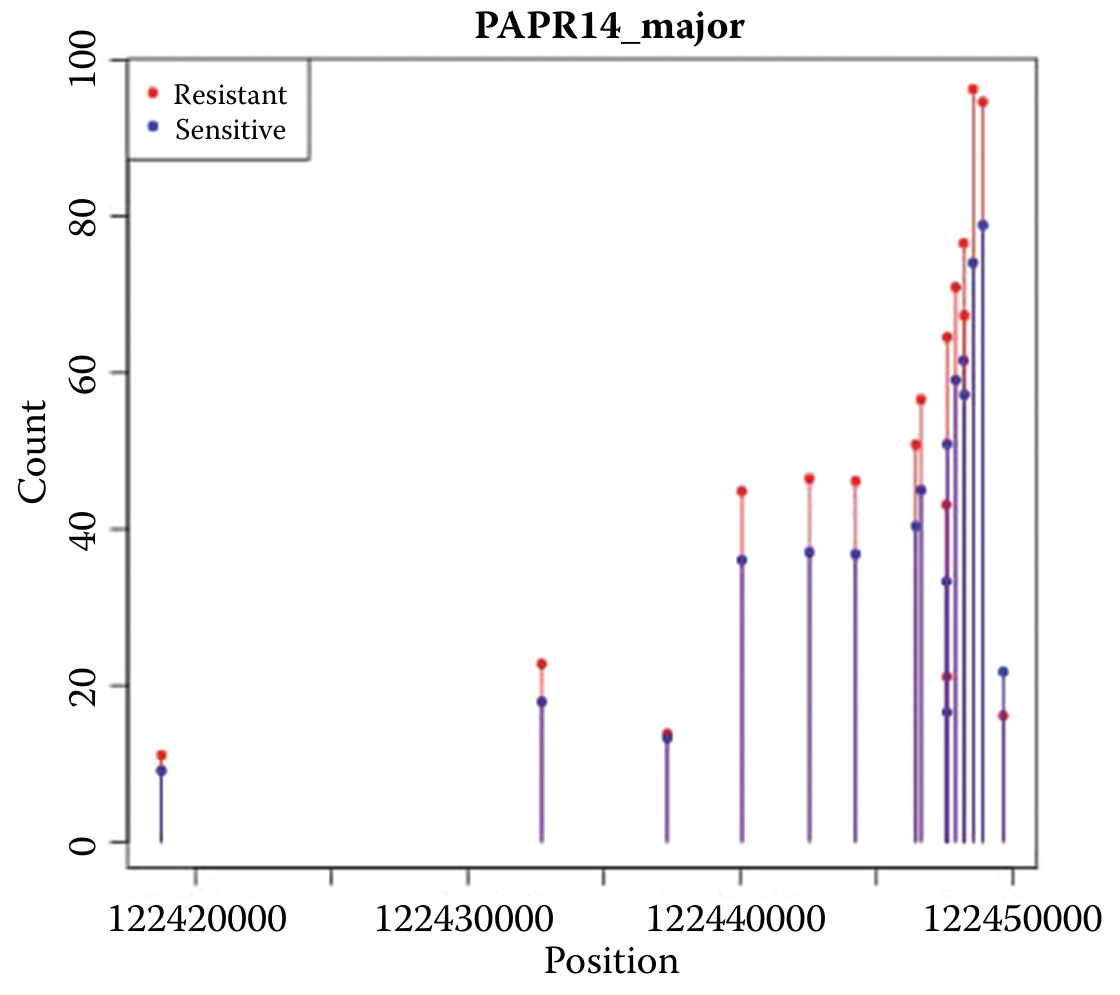
\includegraphics[width=9.8cm]{figures/ch04a_fig16_data.png}};
\fill[white] (4.7291,0.0773) rectangle (5.9744,0.4773);
\node[inner sep=0pt,fill=white,rotate=0,font=\fontsize{8}{8}\selectfont] at (5.3517,0.2773) {位置};
\fill[white] (0.1099,4.2605) rectangle (0.5099,5.2328);
\node[inner sep=0pt,fill=white,rotate=90,font=\fontsize{8}{8}\selectfont] at (0.3099,4.7467) {计数};
\fill[white] (1.4906,7.7027) rectangle (2.5383,8.0152);
\node[inner sep=0pt,fill=white,rotate=0,font=\fontsize{8}{8}\selectfont] at (2.0144,7.8590) {耐药};
\fill[white] (1.5056,7.3967) rectangle (2.5297,7.7092);
\node[inner sep=0pt,fill=white,rotate=0,font=\fontsize{8}{8}\selectfont] at (2.0176,7.5529) {敏感};
\fill[white] (4.1214,8.2613) rectangle (6.5451,8.6613);
\node[inner sep=0pt,fill=white,rotate=0,font=\fontsize{8}{8}\selectfont] at (5.3333,8.4613) {PAPR14：主要等位基因};
\end{tikzpicture}
\origfig{16}{基因 PAPR14 主要等位基因的差异表达。}
\label{fig:ch04a-16}
\end{figure}

\begin{figure}[htbp]
\centering
\begin{tikzpicture}[x=1cm,y=1cm]
\node[anchor=south west,inner sep=0] at (0,0) {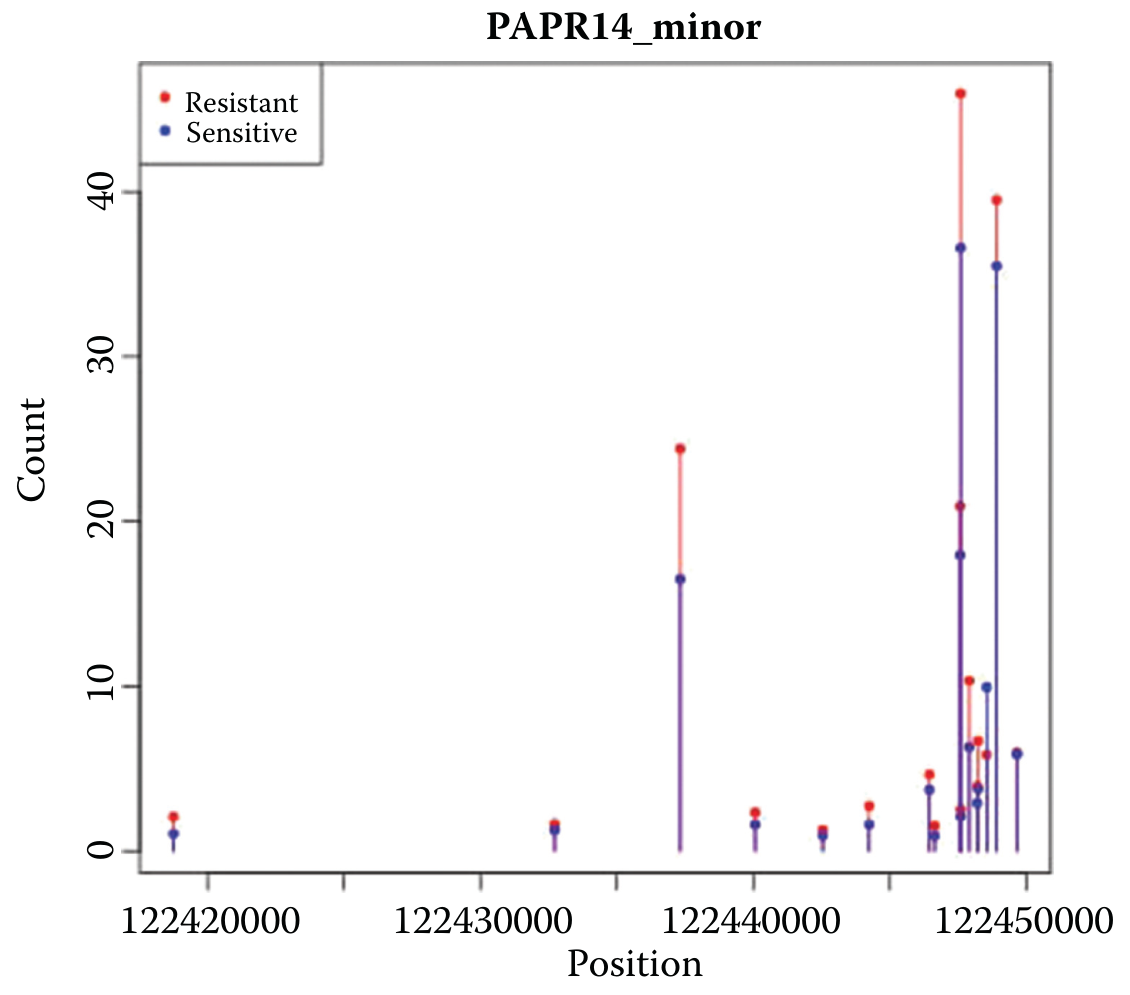
\includegraphics[width=9.8cm]{figures/ch04a_fig17_data.png}};
\fill[white] (4.8892,0.0574) rectangle (6.1237,0.4543);
\node[inner sep=0pt,fill=white,rotate=0,font=\fontsize{8}{8}\selectfont] at (5.5064,0.2558) {位置};
\fill[white] (0.0980,4.2398) rectangle (0.4949,5.2039);
\node[inner sep=0pt,fill=white,rotate=90,font=\fontsize{8}{8}\selectfont] at (0.2964,4.7219) {计数};
\fill[white] (1.5746,7.5693) rectangle (2.6135,7.8794);
\node[inner sep=0pt,fill=white,rotate=0,font=\fontsize{8}{8}\selectfont] at (2.0940,7.7243) {耐药};
\fill[white] (1.5895,7.3089) rectangle (2.6050,7.6191);
\node[inner sep=0pt,fill=white,rotate=0,font=\fontsize{8}{8}\selectfont] at (2.0972,7.4640) {敏感};
\fill[white] (4.1853,8.1811) rectangle (6.6292,8.5780);
\node[inner sep=0pt,fill=white,rotate=0,font=\fontsize{8}{8}\selectfont] at (5.4073,8.3795) {PAPR14：次要等位基因};
\end{tikzpicture}
\origfig{17}{基因 PAPR14 次要等位基因的差异表达。}
\label{fig:ch04a-17}
\end{figure}


这些图呈现出几个特征。第一，等位基因表达水平在不同 SNP 间剧烈变化。复杂的 ASE 模式可能来自可变转录起始或终止位点、等位基因特异性的可变剪接、多个调控变异、生物学变异与测序技术变异。直接将基因内各 SNP 的等位基因读段数相加作为 ASE 总体表达值，或对这些不规则模式建立统计模型进行估计，都并非易事。第二，在基因内许多 SNP 上，主要与次要等位基因的表达水平有显著差异。虽然卵巢癌研究的差异 ASE 检验 $P$ 值并不小，治疗耐药和敏感样本中主要与次要等位基因的表达水平仍有明显差异。第三，在 SLC13A3 的许多 SNP 上，精神分裂症与正常样本间主要和次要等位基因的读段计数均有差异；在 PARP14 的许多 SNP 上，治疗耐药与敏感样本间也如此。

进一步正式检验 SLC13A3 全部 SNP 在精神分裂症与正常样本间的 ASE 差异。表4.9列出了前10个 SNP 的 $P$ 值。单个 SNP 可能只对 ASE 差异作出较小贡献，但它们共同造成了 SLC13A3 在两组间的显著 ASE 差异。这说明，将函数型数据分析用作降维工具，即使采用基于基因型的检验，也能保持较高的功效以发现显著 ASE 差异。
\begin{table}[htbp]
\centering\small
\origtable{9}{基因 SLC13A3 中精神分裂症与正常样本间 ASE 差异检验的前10个 SNP 的 $P$ 值}
\begin{tabular}{lrr}
\toprule
基因组位置&RS 编号&$P$ 值\\
\midrule
44674193&&0.00265\\
44658276&&0.0072\\
44737451&&0.00911\\
44737452&&0.01741\\
44699440&rs6124837&0.02602\\
44620155&rs12617&0.02958\\
44622520&rs910063&0.03634\\
44697695&rs2425889&0.0424\\
44714575&&0.05169\\
44621840&rs4809591&0.05195\\
\bottomrule
\end{tabular}
\end{table}

\FloatBarrier
